\documentclass[border=4mm,multi=tikzpicture]{standalone}
\usepackage[utf8]{inputenc}
\usepackage[T1]{fontenc}
\usepackage[scaled]{helvet}
\renewcommand{\familydefault}{\sfdefault}
\usepackage{amssymb}
\usepackage{xcolor}
\usepackage{tikz}
\usetikzlibrary{positioning, arrows.meta, fit, calc, matrix, backgrounds}
\usepackage[most]{tcolorbox}

\definecolor{accBlue}{HTML}{2563EB}
\definecolor{accGreen}{HTML}{16A34A}
\definecolor{accRed}{HTML}{DC2626}
\definecolor{accOrange}{HTML}{EA580C}
\definecolor{accPurple}{HTML}{7C3AED}
\definecolor{accBlack}{HTML}{1A1A1A}
\definecolor{featTeal}{HTML}{0D9488}
\definecolor{featPink}{HTML}{DB2777}
\definecolor{featAmber}{HTML}{B45309}
\definecolor{featSlate}{HTML}{475569}
\definecolor{panelBg}{HTML}{F7F7F7}
\definecolor{bodyText}{HTML}{333333}
\definecolor{mutedText}{HTML}{666666}

\begin{document}

% ─── DIAGRAM 1: Big model vs matchbox model ───
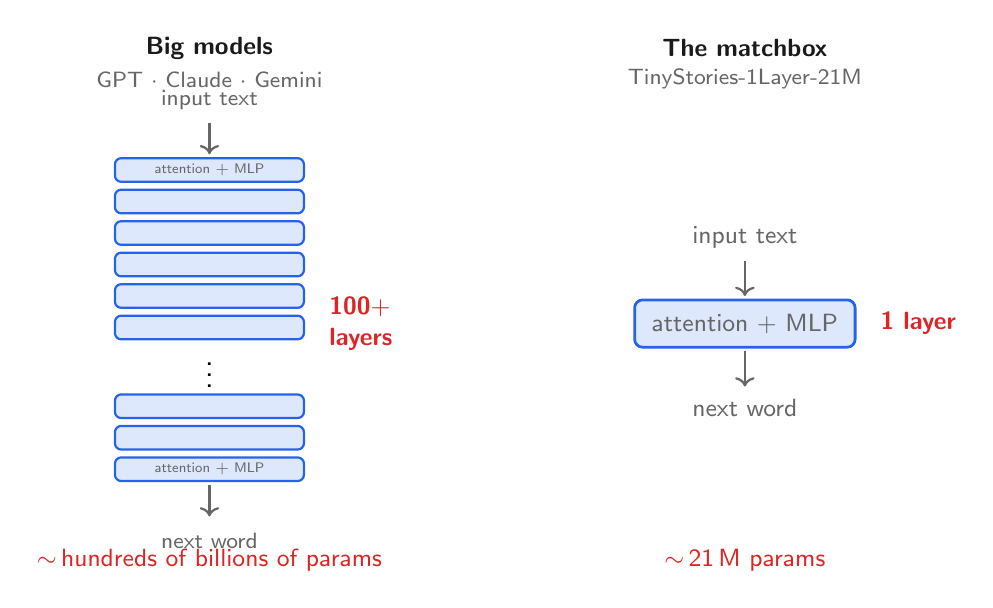
\begin{tikzpicture}[every node/.style={font=\small}]
  % LEFT: big model — stack of layers
  \begin{scope}[xshift=-3.4cm]
    \foreach \y in {0, 0.4, 0.8} {
      \draw[accBlue, fill=accBlue!15, rounded corners=0.8mm, thick]
        (-1.2, \y) rectangle (1.2, \y + 0.3);
    }
    \node[font=\tiny, color=mutedText] at (0, 0.15) {attention $+$ MLP};
    \node at (0, 1.45) {\large $\vdots$};
    \foreach \y in {1.8, 2.2, 2.6, 3.0, 3.4, 3.8} {
      \draw[accBlue, fill=accBlue!15, rounded corners=0.8mm, thick]
        (-1.2, \y) rectangle (1.2, \y + 0.3);
    }
    \node[font=\tiny, color=mutedText] at (0, 3.95) {attention $+$ MLP};
    \draw[->, thick, mutedText] (0, 4.55) -- (0, 4.15);
    \node[font=\footnotesize, color=mutedText, above=1pt] at (0, 4.55) {input text};
    \draw[->, thick, mutedText] (0, -0.05) -- (0, -0.45);
    \node[font=\footnotesize, color=mutedText, below=1pt] at (0, -0.5) {next word};
    \node[right, align=left, color=accRed, font=\small\bfseries] at (1.4, 2) {100$+$\\layers};
    \node[font=\small\bfseries, color=accBlack] at (0, 5.5) {Big models};
    \node[font=\footnotesize, color=mutedText] at (0, 5.1) {GPT $\cdot$ Claude $\cdot$ Gemini};
    \node[font=\small, color=accRed] at (0, -1.0) {$\sim$\,hundreds of billions of params};
  \end{scope}

  % RIGHT: matchbox model — single layer
  \begin{scope}[xshift=3.4cm, yshift=1.7cm]
    \draw[accBlue, fill=accBlue!15, rounded corners=1mm, thick, line width=1pt]
      (-1.4, 0) rectangle (1.4, 0.6);
    \node[color=mutedText, font=\small] at (0, 0.3) {attention $+$ MLP};
    \draw[->, thick, mutedText] (0, 1.1) -- (0, 0.65);
    \node[color=mutedText, above=1pt, font=\small] at (0, 1.1) {input text};
    \draw[->, thick, mutedText] (0, -0.05) -- (0, -0.5);
    \node[color=mutedText, below=1pt, font=\small] at (0, -0.5) {next word};
    \node[right, align=left, color=accRed, font=\small\bfseries] at (1.6, 0.3) {1 layer};
    \node[font=\small\bfseries, color=accBlack] at (0, 3.8) {The matchbox};
    \node[font=\footnotesize, color=mutedText] at (0, 3.4) {TinyStories-1Layer-21M};
    \node[font=\small, color=accRed] at (0, -2.7) {$\sim$\,21\,M params};
  \end{scope}
\end{tikzpicture}

% ─── DIAGRAM 2: Model diagram with 16 heads (English) ───
\newcommand{\modeldiag}{%
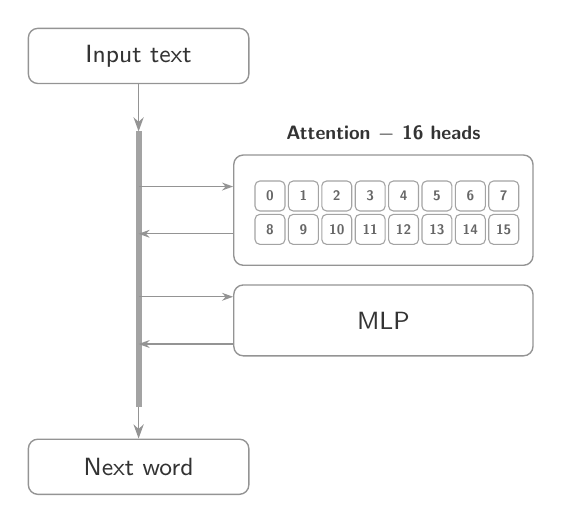
\begin{tikzpicture}[
  every node/.style={font=\small},
  endbox/.style={rectangle, rounded corners=1.2mm, draw=mutedText!70, line width=0.5pt,
              text=bodyText, minimum width=28mm, minimum height=7mm,
              align=center, font=\small, inner sep=1mm},
  sidebox/.style={rectangle, rounded corners=1.2mm, draw=mutedText!70, line width=0.5pt,
              text=bodyText, minimum width=28mm, minimum height=9mm,
              align=center, font=\small, inner sep=1mm},
  hd/.style={rectangle, rounded corners=0.6mm, draw=mutedText!60, line width=0.4pt,
             text=mutedText, minimum width=3.8mm, minimum height=3.8mm,
             font=\tiny\bfseries, inner sep=0pt},
  stream/.style={draw=mutedText!60, line width=2.2pt},
  tap/.style={->, >={Stealth[length=1.4mm, width=1mm]}, mutedText!70, line width=0.5pt},
  arrv/.style={->, >={Stealth[length=1.8mm, width=1.3mm]}, mutedText!70, line width=0.5pt},
]
  \coordinate (spine_top)   at (0,  -5mm);
  \coordinate (attn_in)     at (0, -12mm);
  \coordinate (attn_out)    at (0, -18mm);
  \coordinate (mlp_in)      at (0, -26mm);
  \coordinate (mlp_out)     at (0, -32mm);
  \coordinate (spine_bot)   at (0, -40mm);

  \node[endbox, anchor=south] at (0, 1mm) (in) {Input text};
  \node[endbox, anchor=north] at (0, -44mm) (out) {Next word};
  \draw[stream] (spine_top) -- (spine_bot);

  \node[sidebox, minimum height=14mm, minimum width=38mm, anchor=west]
        at (12mm, -15mm) (attn) {};
  \node[above=0.3mm of attn.north, font=\scriptsize\bfseries, color=bodyText]
        {Attention $-$ 16 heads};

  \node[hd, anchor=center] at ($(attn.center) + (-14.4mm, 1.8mm)$) (h0) {0};
  \node[hd, right=0.3mm of h0]  (h1)  {1};
  \node[hd, right=0.3mm of h1]  (h2)  {2};
  \node[hd, right=0.3mm of h2]  (h3)  {3};
  \node[hd, right=0.3mm of h3]  (h4)  {4};
  \node[hd, right=0.3mm of h4]  (h5)  {5};
  \node[hd, right=0.3mm of h5]  (h6)  {6};
  \node[hd, right=0.3mm of h6]  (h7)  {7};
  \node[hd, below=0.3mm of h0]  (h8)  {8};
  \node[hd, right=0.3mm of h8]  (h9)  {9};
  \node[hd, right=0.3mm of h9]  (h10) {10};
  \node[hd, right=0.3mm of h10] (h11) {11};
  \node[hd, right=0.3mm of h11] (h12) {12};
  \node[hd, right=0.3mm of h12] (h13) {13};
  \node[hd, right=0.3mm of h13] (h14) {14};
  \node[hd, right=0.3mm of h14] (h15) {15};

  \draw[tap] (attn_in)  -- (attn.west |- attn_in);
  \draw[tap] (attn.west |- attn_out) -- (attn_out);

  \node[sidebox, minimum width=38mm, anchor=west] at (12mm, -29mm) (mlp) {MLP};
  \draw[tap] (mlp_in) -- (mlp.west |- mlp_in);
  \draw[tap] (mlp.west |- mlp_out) -- (mlp_out);

  \draw[arrv] (in.south) -- (spine_top);
  \draw[arrv] (spine_bot) -- (out.north);
\end{tikzpicture}%
}
\modeldiag

% ─── DIAGRAM 3: LoRA W + B·A ───
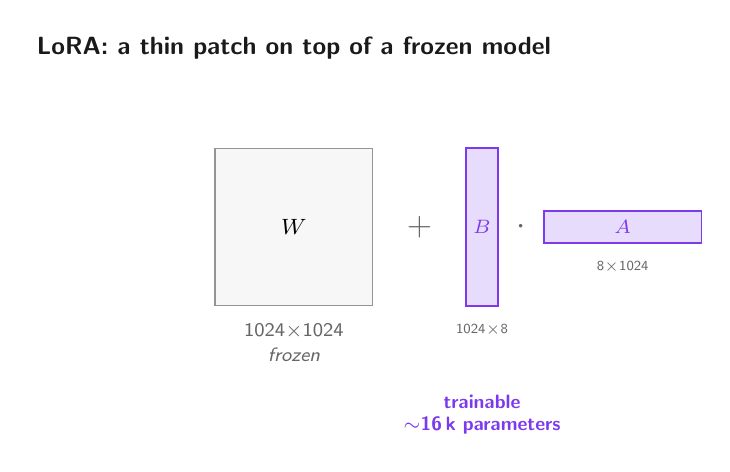
\begin{tikzpicture}[
  every node/.style={font=\footnotesize},
  bigW/.style={rectangle, draw=mutedText!70, line width=0.5pt, fill=panelBg,
               minimum width=20mm, minimum height=20mm, align=center},
  thinB/.style={rectangle, draw=accPurple, line width=0.6pt, fill=accPurple!18,
                minimum width=4mm, minimum height=20mm, align=center},
  thinA/.style={rectangle, draw=accPurple, line width=0.6pt, fill=accPurple!18,
                minimum width=20mm, minimum height=4mm, align=center},
  op/.style={font=\large\bfseries, color=mutedText},
]
  \node[bigW] (W) {$W$};
  \node[below=1mm of W, font=\scriptsize\color{mutedText}] {1024$\times$1024};
  \node[below=4mm of W, font=\scriptsize\color{mutedText}\itshape] {frozen};

  \node[op, right=3mm of W] (plus) {$+$};

  \node[thinB, right=3mm of plus] (B) {};
  \node[font=\scriptsize, color=accPurple] at (B) {$B$};
  \node[below=1mm of B, font=\tiny\color{mutedText}] {1024$\times$8};

  \node[op, right=1mm of B] (mul) {$\cdot$};

  \node[thinA, right=1mm of mul, anchor=west] (A) {};
  \node[font=\scriptsize, color=accPurple] at (A) {$A$};
  \node[below=1mm of A, font=\tiny\color{mutedText}] {8$\times$1024};

  \node[below=10mm of B, font=\scriptsize\bfseries\color{accPurple}, align=center]
        {trainable\\$\sim$16\,k parameters};
  \node[above=10mm of W, font=\small\bfseries\color{accBlack}, align=center]
        {LoRA: a thin patch on top of a frozen model};
\end{tikzpicture}

% ─── DIAGRAM 4: 64 styles — book → book with LoRA glow ───
\begin{tikzpicture}[every node/.style={font=\footnotesize}]
  \node[anchor=north] at (-4.5, 4) {%
    
\includegraphics[height=2.4cm,keepaspectratio]{../presentation_assets/images/tinystories.png}};
  \node[font=\footnotesize, color=mutedText, anchor=north, align=center] at (-4.5, 0.6)
        {\itshape children's\\ \itshape stories};

  \node[draw=mutedText!50, rounded corners=1mm, line width=0.4pt, fill=panelBg,
        inner sep=1mm, anchor=north] (lbox) at (-4.5, -0.7) {%
    \begin{tikzpicture}[hd/.style={rectangle, rounded corners=0.3mm, draw=mutedText!60,
                        line width=0.3pt, minimum width=4.0mm, minimum height=4.0mm,
                        inner sep=0pt, text=mutedText, font=\tiny\bfseries}]
      \foreach \i in {0,...,7} { \node[hd] at (\i*4.3mm, 0) {\i}; }
      \foreach \i [evaluate=\i as \n using int(\i+8)] in {0,...,7}
        { \node[hd] at (\i*4.3mm, -4.3mm) {\n}; }
    \end{tikzpicture}};
  \node[below=0.5mm of lbox, font=\tiny\color{mutedText}\itshape] {16 attention heads};

  \node[font=\Large, color=accBlue] at (0, 2.5) {$\to$};
  \node[font=\scriptsize, color=mutedText, align=center] at (0, 1.9) {LoRA\\$\sim$0.26\,\% of weights};

  \node[anchor=north] at (4.5, 4) {%
    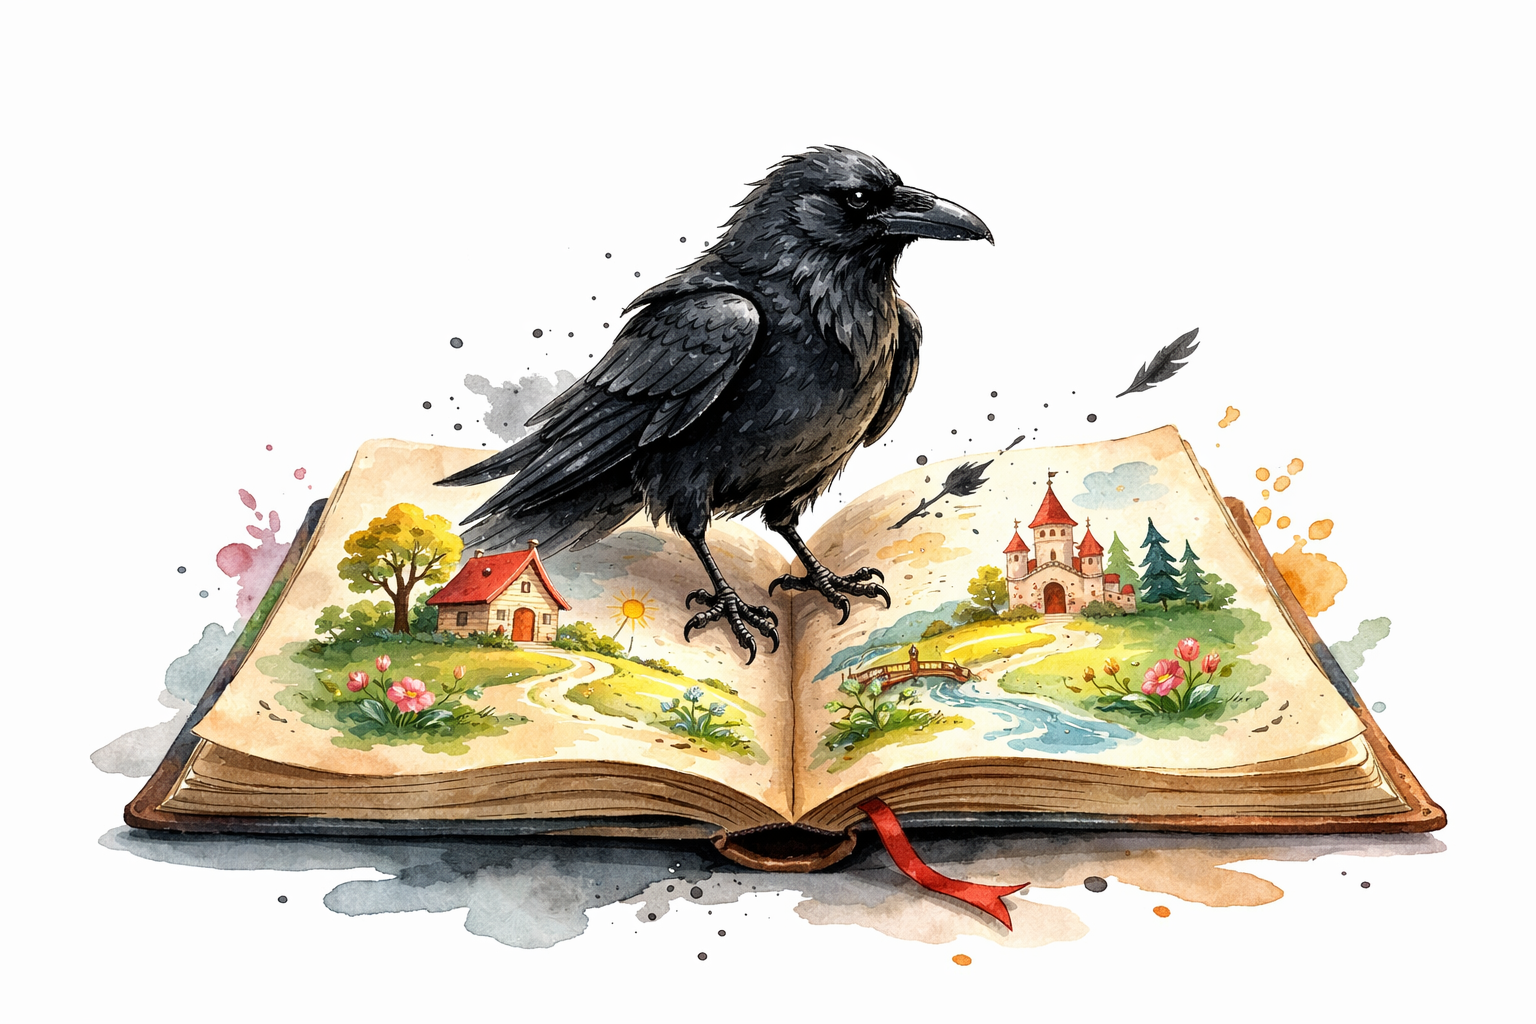
\includegraphics[height=2.4cm,keepaspectratio]{../presentation_assets/images/sixteen_voices.png}};
  \node[font=\footnotesize, color=mutedText, anchor=north, align=center] at (4.5, 0.6)
        {\itshape e.g.\ Poe};

  \node[draw=mutedText!50, rounded corners=1mm, line width=0.4pt, fill=panelBg,
        inner sep=1mm, anchor=north] (rbox) at (4.5, -0.7) {%
    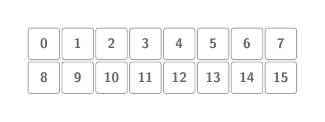
\begin{tikzpicture}[hd/.style={rectangle, rounded corners=0.3mm, draw=mutedText!60,
                        line width=0.3pt, minimum width=4.0mm, minimum height=4.0mm,
                        inner sep=0pt, text=mutedText, font=\tiny\bfseries}]
      \foreach \i in {0,...,7} { \node[hd] at (\i*4.3mm, 0) {\i}; }
      \foreach \i [evaluate=\i as \n using int(\i+8)] in {0,...,7}
        { \node[hd] at (\i*4.3mm, -4.3mm) {\n}; }
    \end{tikzpicture}};
  \begin{scope}[on background layer]
    \node[draw=accPurple, line width=0.3pt, fill=accPurple!8,
          rounded corners=1.6mm, inner sep=1.6mm, fit=(rbox)] {};
    \node[draw=accPurple!50, line width=0.25pt, fill=accPurple!4,
          rounded corners=2.4mm, inner sep=2.4mm, fit=(rbox)] {};
    \node[draw=accPurple!25, line width=0.2pt,
          rounded corners=3.2mm, inner sep=3.2mm, fit=(rbox)] (glow) {};
  \end{scope}
  \node[below=0.5mm of glow, font=\tiny\color{accPurple}\bfseries\itshape, align=center]
        {$+$ LoRA adapter $-$ wakes up the style};

  \node[font=\bfseries, color=accBlack] at (0, 4.5) {64 styles in a matchbox};
\end{tikzpicture}

% ─── DIAGRAM 5: SAE prism ───
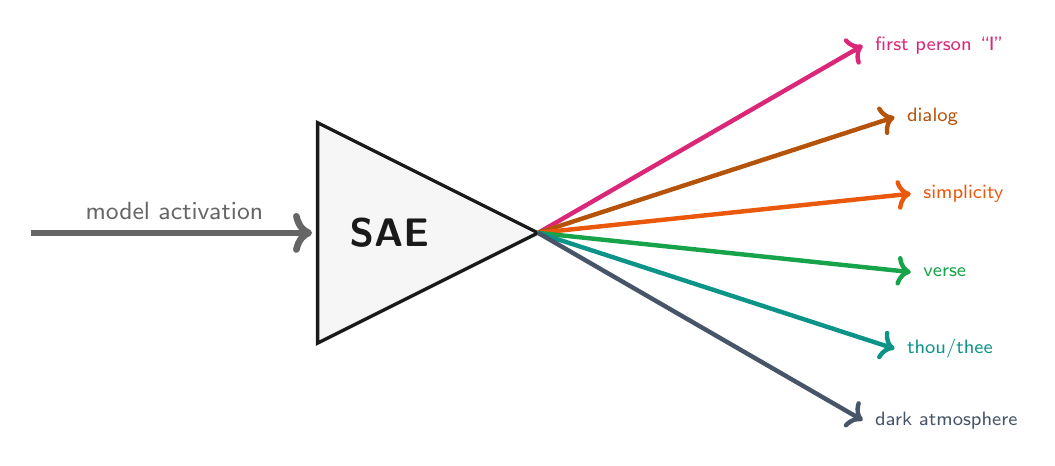
\begin{tikzpicture}[scale=1.4]
  \draw[->, line width=2.4pt, color=mutedText] (-3.6, 0) -- (-1.05, 0);
  \node[font=\small, color=mutedText, above=0.5mm] at (-2.3, 0) {model activation};
  \draw[line width=1.2pt, color=accBlack, fill=accBlack!4]
    (-1.0, -1.0) -- (1.0, 0) -- (-1.0, 1.0) -- cycle;
  \node[font=\Large\bfseries, color=accBlack] at (-0.35, 0) {SAE};
  \def\beamlen{3.4}
  \foreach \angle/\col in {30/featPink, 18/featAmber, 6/accOrange, -6/accGreen, -18/featTeal, -30/featSlate} {
    \draw[->, line width=1.6pt, color=\col]
      (1.0, 0) -- ({1.0 + \beamlen*cos(\angle)}, {\beamlen*sin(\angle)});
  }
  \node[font=\scriptsize, color=featPink, right=1pt] at ({1.0 + \beamlen*cos(30)}, {\beamlen*sin(30)}) {first person ``I''};
  \node[font=\scriptsize, color=featAmber, right=1pt] at ({1.0 + \beamlen*cos(18)}, {\beamlen*sin(18)}) {dialog};
  \node[font=\scriptsize, color=accOrange, right=1pt] at ({1.0 + \beamlen*cos(6)}, {\beamlen*sin(6)}) {simplicity};
  \node[font=\scriptsize, color=accGreen, right=1pt] at ({1.0 + \beamlen*cos(-6)}, {\beamlen*sin(-6)}) {verse};
  \node[font=\scriptsize, color=featTeal, right=1pt] at ({1.0 + \beamlen*cos(-18)}, {\beamlen*sin(-18)}) {thou/thee};
  \node[font=\scriptsize, color=featSlate, right=1pt] at ({1.0 + \beamlen*cos(-30)}, {\beamlen*sin(-30)}) {dark atmosphere};
\end{tikzpicture}

% ─── DIAGRAM 6: Poe scaling 0x / 1x / 2x ───
\begin{tikzpicture}[every node/.style={font=\small}]
  \node[anchor=north] at (-4.6, 3) {%
    
\includegraphics[height=3.0cm,keepaspectratio]{../presentation_assets/images/sixteen_voices_0poe.png}};
  \node[anchor=north] at (0, 3) {%
    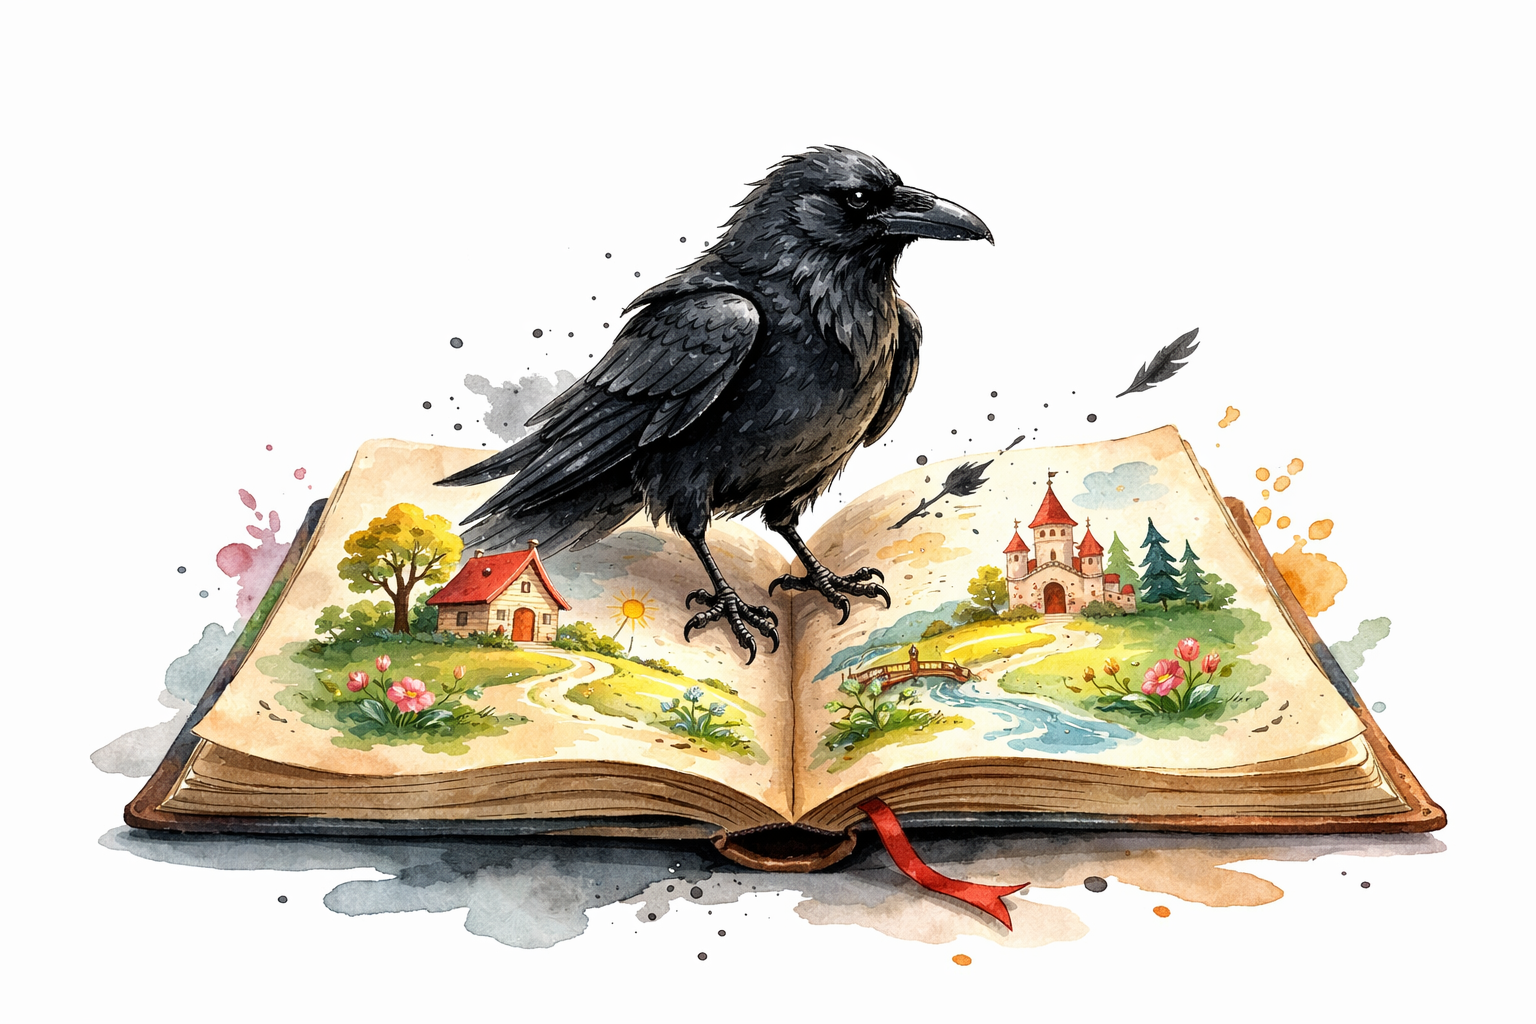
\includegraphics[height=3.0cm,keepaspectratio]{../presentation_assets/images/sixteen_voices.png}};
  \node[anchor=north] at (4.6, 3) {%
    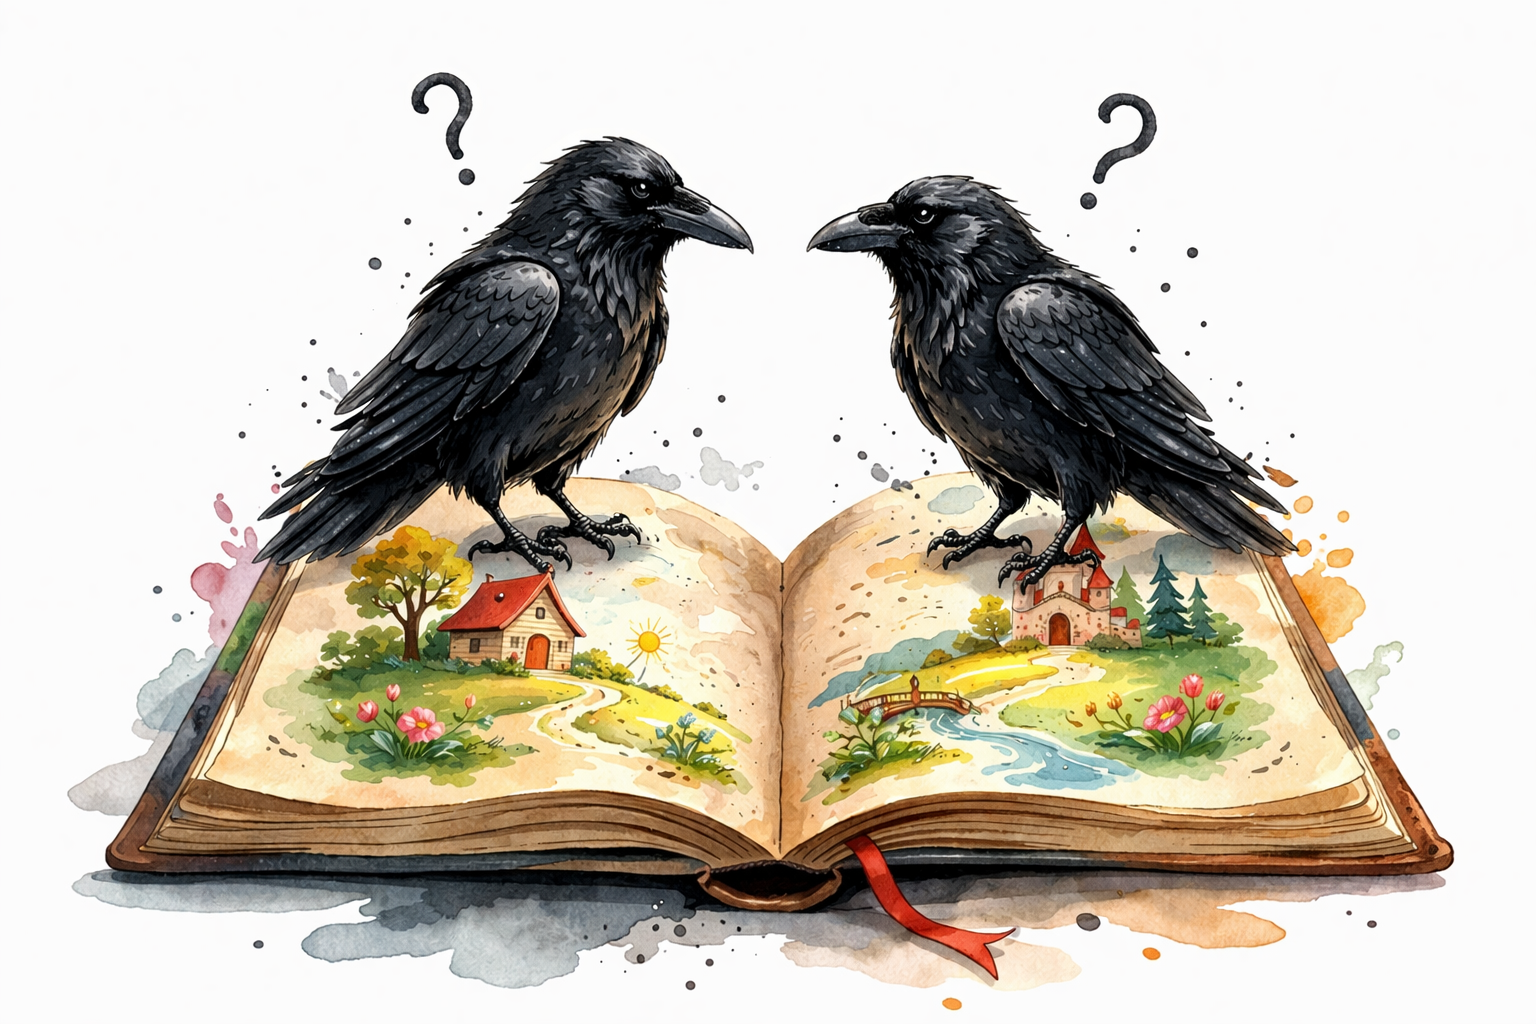
\includegraphics[height=3.0cm,keepaspectratio]{../presentation_assets/images/sixteen_voices_2poe.png}};

  \node[font=\bfseries, color=accBlue] at (-4.6, -0.6) {0$\times$};
  \node[font=\bfseries, color=accGreen] at (0, -0.6) {1$\times$};
  \node[font=\bfseries, color=accRed] at (4.6, -0.6) {2$\times$};

  \node[font=\footnotesize, color=mutedText, align=center] at (-4.6, -1.2) {style breaks};
  \node[font=\footnotesize, color=mutedText, align=center] at (0, -1.2) {sweet spot};
  \node[font=\footnotesize, color=mutedText, align=center] at (4.6, -1.2) {Poe falls apart};

  \node[font=\bfseries, color=accBlack] at (0, 4) {Scaling Poe's dominant head};
\end{tikzpicture}

\end{document}
